\chapter{Manual de usuario}

Este manual describe el funcionamiento de \textit{NeuroForge} y guía al jugador a través de todas las pantallas y mecánicas del videojuego. Toda la interacción se puede realizar solamente con el ratón.

% ─────────────────────────────────────────────────────────────────────────────
\section{Menú principal}
% ─────────────────────────────────────────────────────────────────────────────

Al iniciar el videojuego se muestra el menú principal (Figura~\ref{fig:ManualMenuPrincipal}), desde el que se puede acceder a las tres opciones disponibles: \textit{Play}, para comenzar una nueva partida; \textit{Rules}, para consultar las reglas del videojuego; y \textit{Exit}, para cerrar la aplicación.

\begin{figure}[H]
	\centering
	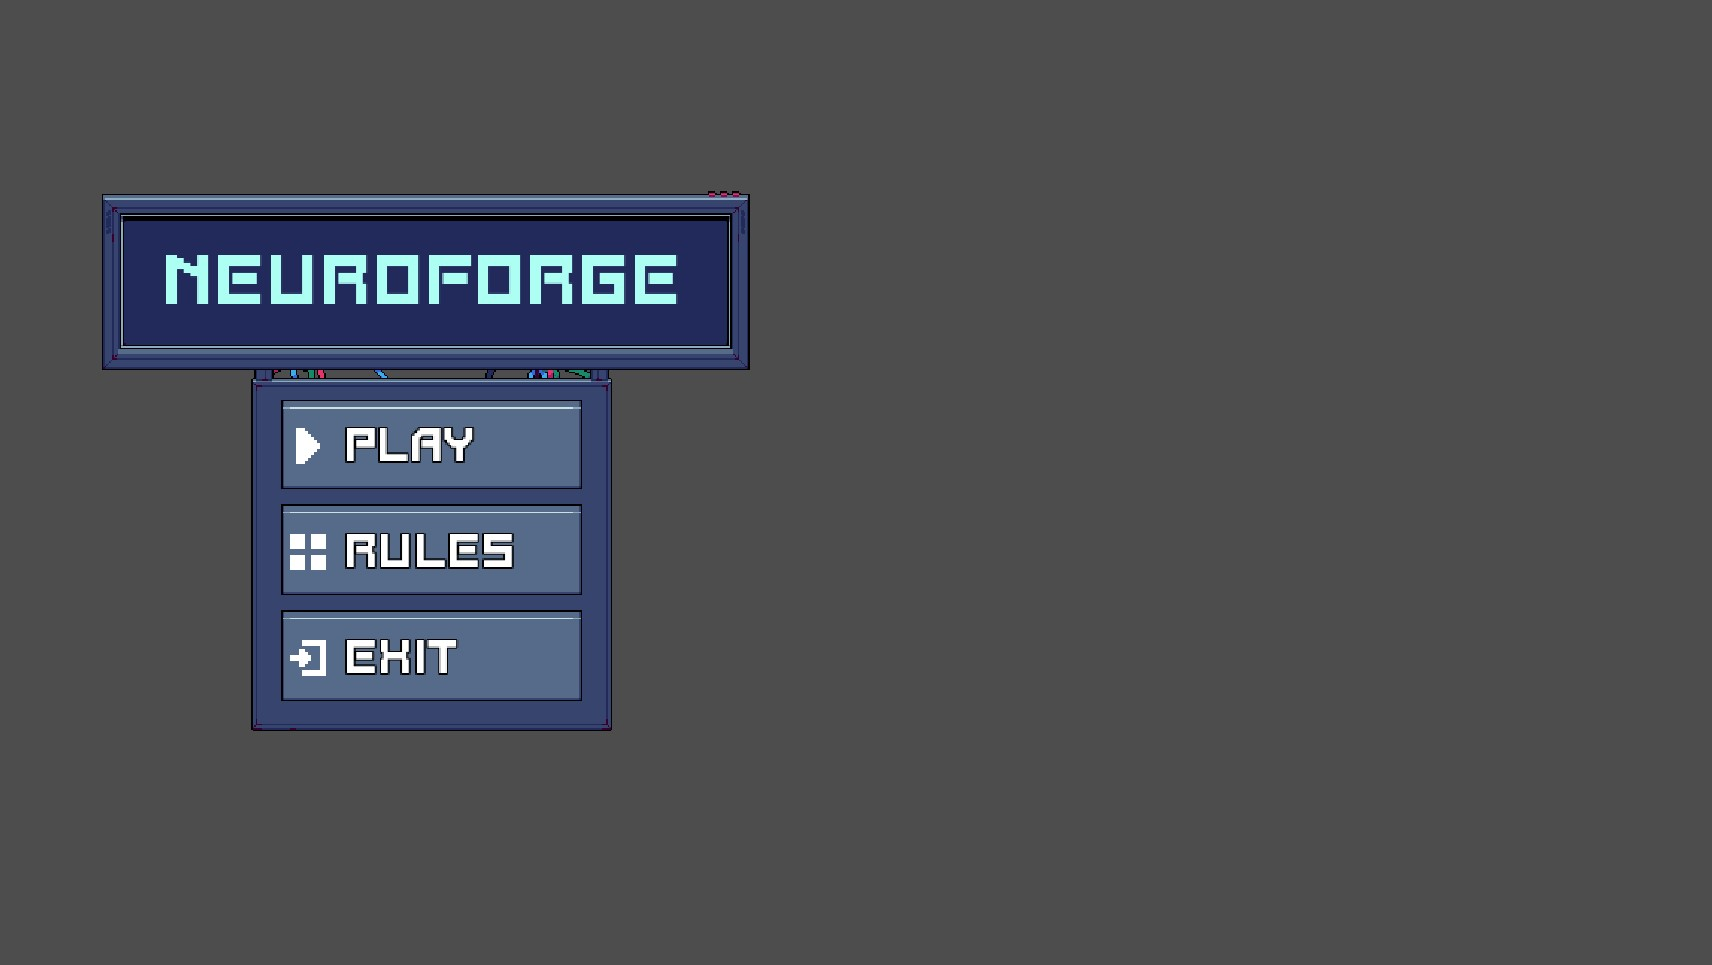
\includegraphics[width=\textwidth]{../Imagenes/MenuPrincipal}
	\caption{Menú principal de NeuroForge.}
	\label{fig:ManualMenuPrincipal}
\end{figure}

% ─────────────────────────────────────────────────────────────────────────────
\section{Menú de reglas}
% ─────────────────────────────────────────────────────────────────────────────

El menú de reglas es accesible tanto desde el menú principal como desde el menú de pausa durante una partida. Se organiza en cinco pestañas navegables en la parte superior de la ventana: \textit{Objective}, con el objetivo y las condiciones de victoria; \textit{Board}, con los tipos de casillas del tablero; \textit{Movement}, con las reglas de desplazamiento; \textit{Combat}, con la mecánica de enfrentamiento; y \textit{Pieces}, que permite consultar el rango, la movilidad
y las reglas especiales de cada tipo de pieza pulsando sobre su botón correspondiente. Para cerrar el menú se pulsa el botón \textit{Go Back} en la esquina superior izquierda.

% ─────────────────────────────────────────────────────────────────────────────
\section{Fase de despliegue}
% ─────────────────────────────────────────────────────────────────────────────

Antes de comenzar la partida, el jugador debe colocar todas sus piezas en su zona de despliegue, las cuatro filas más próximas al borde inferior del tablero. La Figura~\ref{fig:ManualMenuDespliegue} muestra esta pantalla con algunas piezas ya colocadas, con los elementos principales numerados.

Para colocar una pieza manualmente, se pulsa sobre su botón en el panel lateral izquierdo (\textbf{3}) para seleccionarla (\textbf{4}) y a continuación se hace clic sobre cualquier casilla de despliegue del jugador (\textbf{10}). Si se hace clic sobre una pieza ya colocada en el tablero (\textbf{9}), esta se retira y su tipo vuelve a quedar seleccionado en el panel para reposicionarla. Cuando se han colocado todas las unidades de un tipo, el botón correspondiente aparece desactivado (\textbf{5}). El contador en la parte superior del panel (\textbf{1}) indica cuántas piezas quedan todavía por colocar.

El botón de \textit{Despliegue aleatorio} (\textbf{6}) distribuye automáticamente todas las piezas restantes en posiciones aleatorias dentro de la zona de despliegue. Una vez colocadas todas las piezas, el botón de \textit{Comenzar partida} (\textbf{7}) se activa y al pulsarlo el bot despliega sus piezas en su zona (\textbf{8}) y comienza la partida.

\clearpage

\begin{figure}[H]
	\centering
	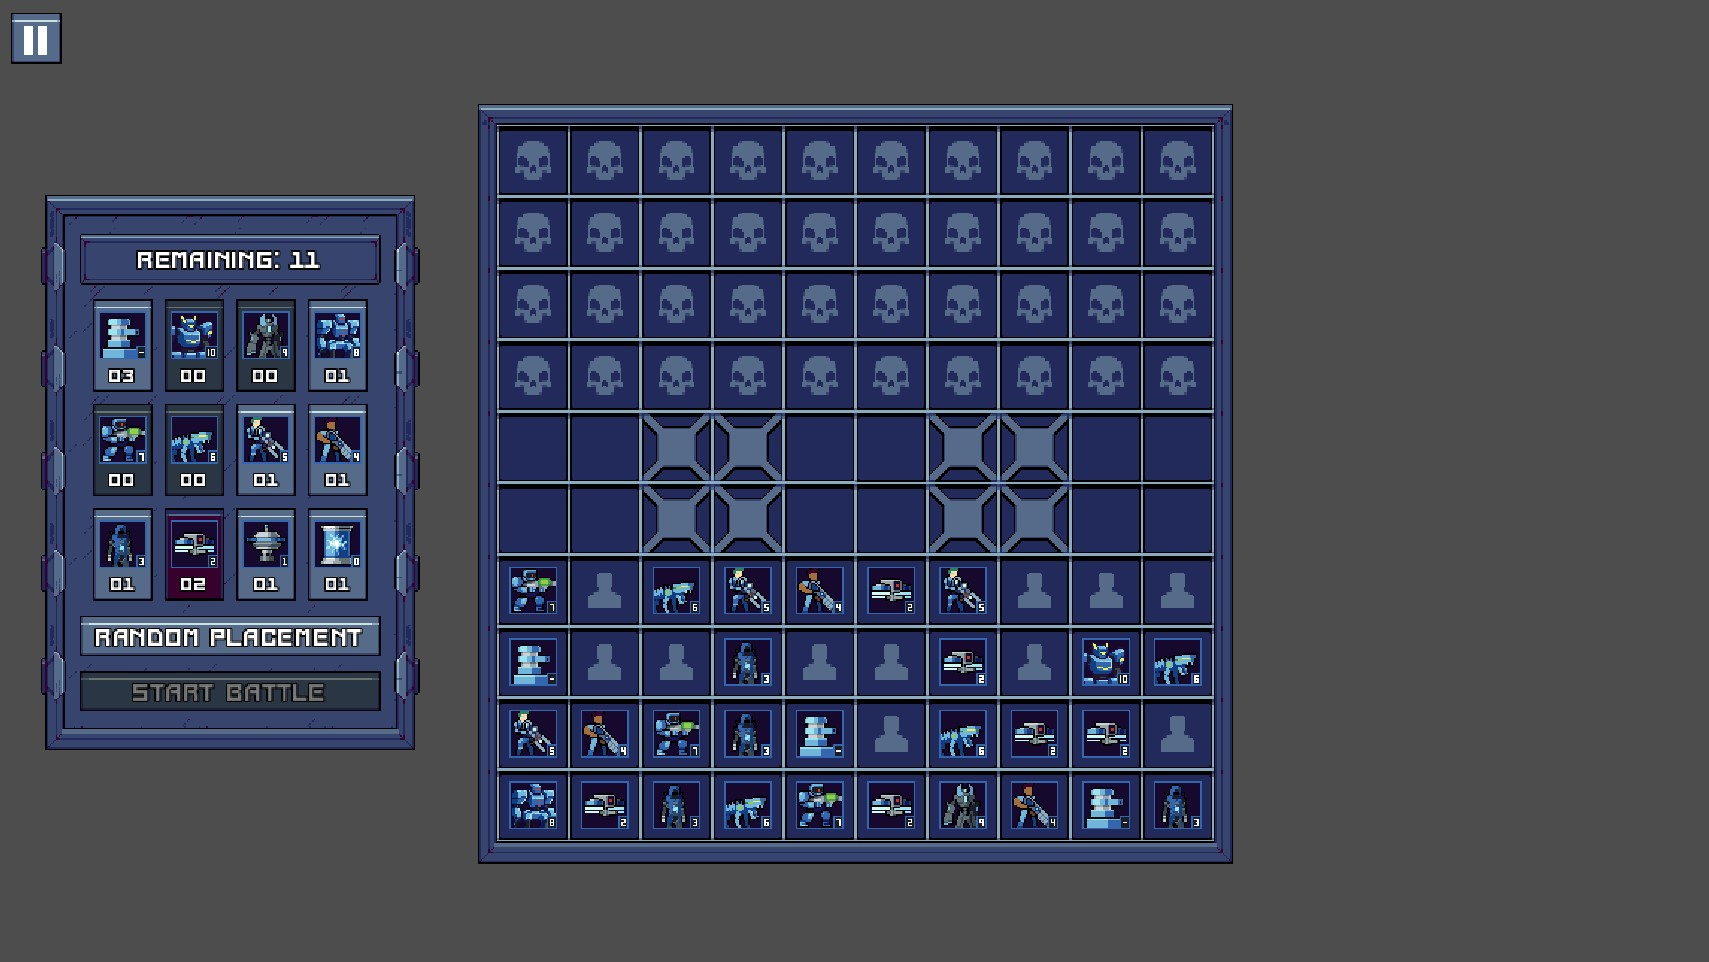
\includegraphics[width=\textwidth]{../Imagenes/MenuDespliegueParcialmenteVacio}
	\caption{Fase de despliegue con algunas piezas ya colocadas en la zona del jugador.}
	\label{fig:ManualMenuDespliegue}
\end{figure}

\begin{enumerate}
	\item \textbf{Panel de despliegue:} Indica las piezas totales que quedan por colocar.
	\item \textbf{Tablero:} Zona donde desplegar las piezas seleccionadas.
	\item \textbf{Pieza pendiente por colocar:} Botón con contador individual que muestra cuántas unidades de ese tipo quedan por colocar.
	\item \textbf{Pieza seleccionada:} Tipo de pieza activo que se colocará en la siguiente casilla válida en la que se haga clic.
	\item \textbf{Pieza agotada:} Tipo del que ya se han colocado todas las unidades disponibles.
	\item \textbf{Botón de despliegue aleatorio:} Distribuye aleatoriamente todas las piezas restantes en la zona de despliegue del jugador.
	\item \textbf{Botón de inicio de partida:} Inicia la partida. Permanece desactivado mientras queden piezas por colocar.
	\item \textbf{Casilla de despliegue del bot:} Zona reservada al bot; sus piezas se colocan aquí automáticamente al pulsar \textit{Start Battle}.
	\item \textbf{Pieza desplegada:} Pieza ya colocada en el tablero. Al hacer clic sobre ella se retira y su tipo vuelve a quedar seleccionado en el panel.
	\item \textbf{Casilla de despliegue del jugador:} Casillas donde el jugador puede colocar sus piezas.
\end{enumerate}

% ─────────────────────────────────────────────────────────────────────────────
\section{Partida en curso}
% ─────────────────────────────────────────────────────────────────────────────

La partida se desarrolla en turnos alternos, comenzando siempre el jugador. Al inicio de cada turno del jugador, las piezas que tienen algún movimiento disponible aparecen ligeramente resaltadas para identificarlas de un vistazo. Al hacer clic sobre una de ellas, el tablero muestra en verde las casillas a las que puede desplazarse (\textbf{3}) y en rojo las casillas ocupadas por piezas enemigas a las que puede atacar (\textbf{2}), tal como se aprecia en la Figura~\ref{fig:ManualMenuPartida}. Haciendo clic sobre una casilla resaltada se confirma la acción. Para cancelar la selección basta con hacer clic fuera de las casillas resaltadas.

Si la pieza se mueve a una casilla vacía, el turno pasa automáticamente al bot. Si se mueve a una casilla ocupada por una pieza enemiga, se inicia un combate y aparece la interfaz de resolución. El bot ejecuta su turno de forma automática y sin intervención del jugador.

El panel lateral izquierdo (\textbf{1}) muestra en todo momento el recuento de piezas restantes de cada bando. El marcador de turno (\textbf{7}) situado a la derecha muestra un icono de persona durante el turno del jugador y una calavera durante el del bot. Las piezas propias cuya identidad ya conoce el bot aparecen rodeadas por un borde naranja (\textbf{8}), lo que ocurre cuando han sobrevivido a un combate o han realizado un movimiento que revela su tipo.

\begin{figure}[H]
	\centering
	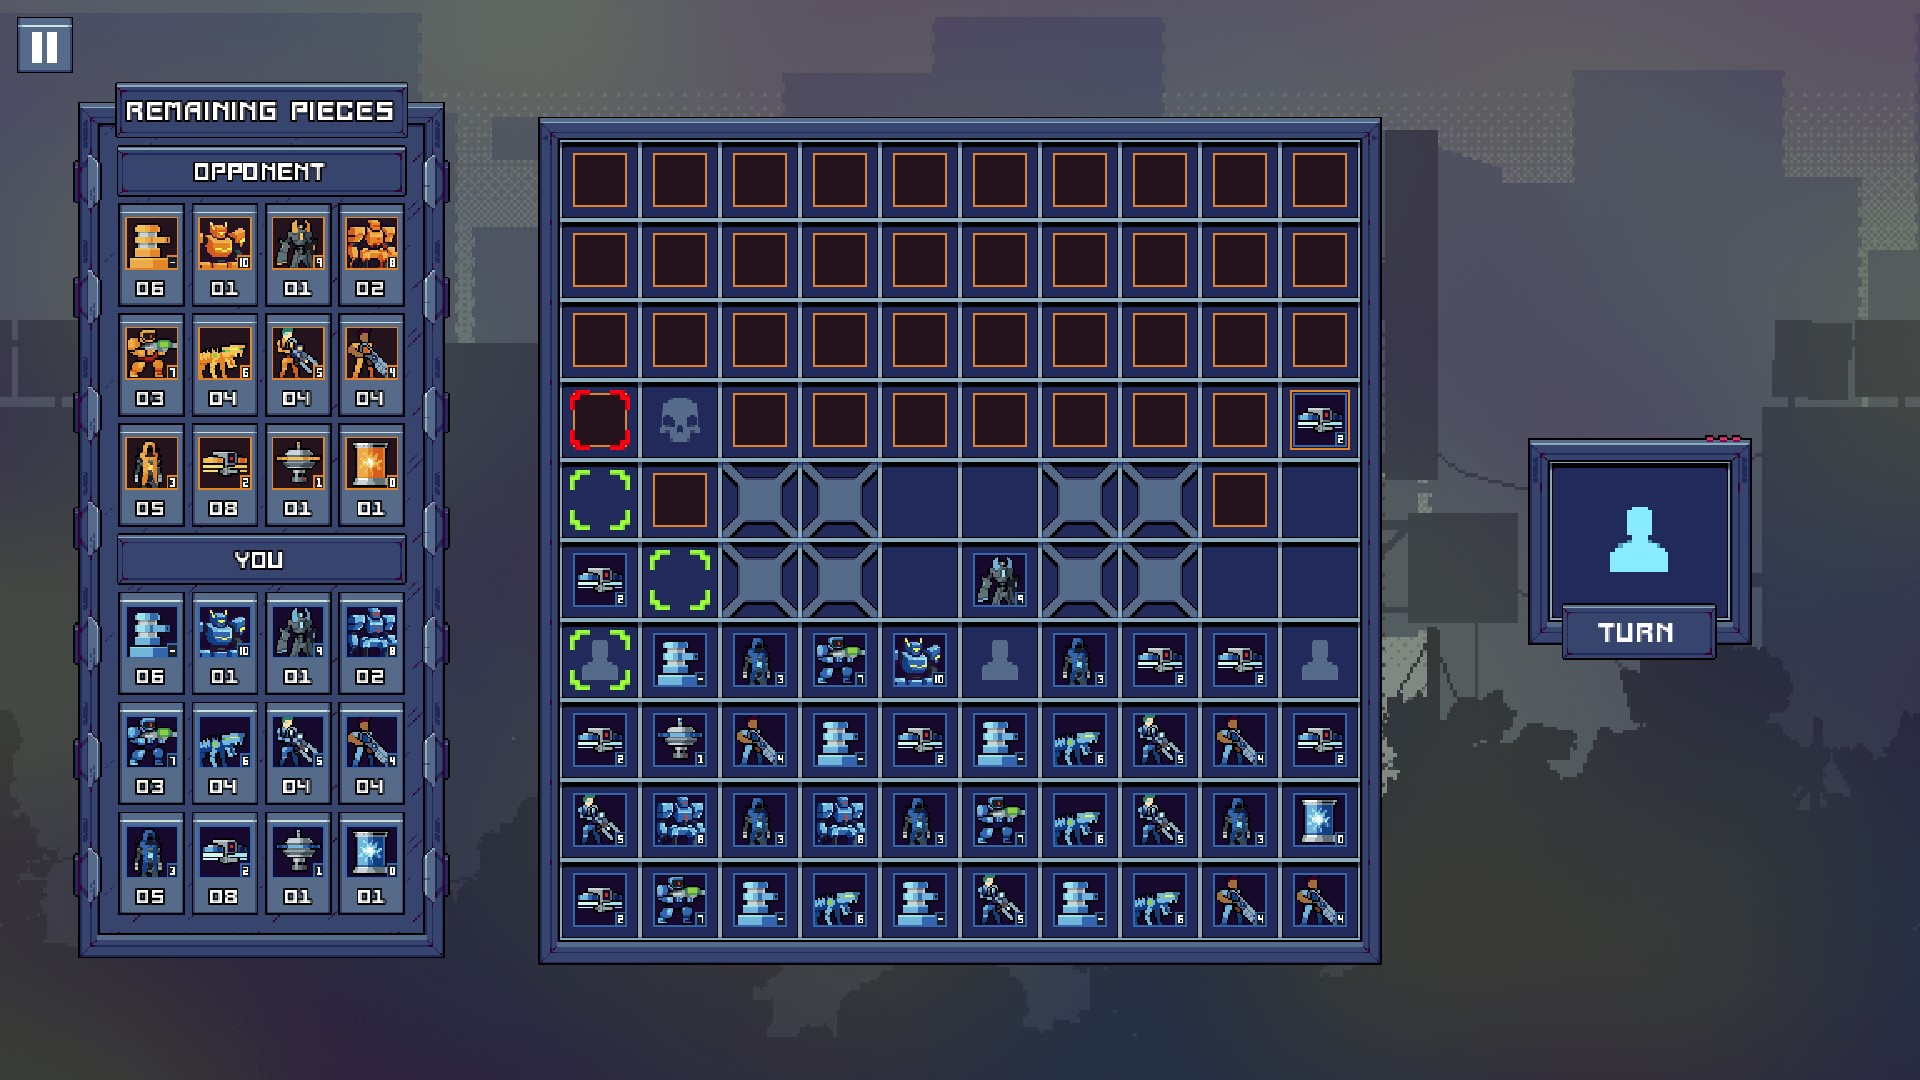
\includegraphics[width=\textwidth]{../Imagenes/MenuPartidaEnCurso}
	\caption{Pantalla de partida con una pieza seleccionada y sus acciones
		posibles resaltadas.}
	\label{fig:ManualMenuPartida}
\end{figure}

\begin{enumerate}
	\item \textbf{Panel de piezas:} Recuento de piezas restantes de ambos bandos, útil para llevar la cuenta de qué tipos quedan en juego.
	\item \textbf{Casilla marcada para combate:} Casilla ocupada por una pieza enemiga a la que la pieza seleccionada puede atacar; se resalta en rojo.
	\item \textbf{Casilla marcada para movimiento:} Casilla libre a la que la pieza seleccionada puede desplazarse; se resalta en verde.
	\item \textbf{Pieza seleccionada:} Pieza activa cuyas casillas de acción quedan resaltadas al hacer clic sobre ella.
	\item \textbf{Casilla transitable:} Casilla por la que se pueden mover las piezas.
	\item \textbf{Casilla intransitable:} Casilla que ninguna pieza puede atravesar ni ocupar.
	\item \textbf{Marcador de turno:} Indica de quién es el turno: icono de persona para el jugador, calavera para el bot.
	\item \textbf{Pieza revelada para el bot:} Pieza propia cuya identidad ya conoce el bot, indicada por un borde naranja.
\end{enumerate}

% ─────────────────────────────────────────────────────────────────────────────
\section{Interfaz de combate}
% ─────────────────────────────────────────────────────────────────────────────

Cuando dos piezas se enfrentan, aparece la ventana de combate que se muestra en la Figura~\ref{fig:ManualMenuCombate}. El atacante aparece a la izquierda, marcado con un icono de mira roja, y el defensor a la derecha, identificado con un escudo azul. Si alguna de las piezas era desconocida para el rival, su sprite parpadea y se revela en este momento. A continuación, la pieza o piezas perdedoras se oscurecen y en la parte inferior aparece un mensaje indicando quién ha ganado y el motivo. Para continuar la partida basta con hacer clic en cualquier punto de la ventana.

\begin{figure}[H]
	\centering
	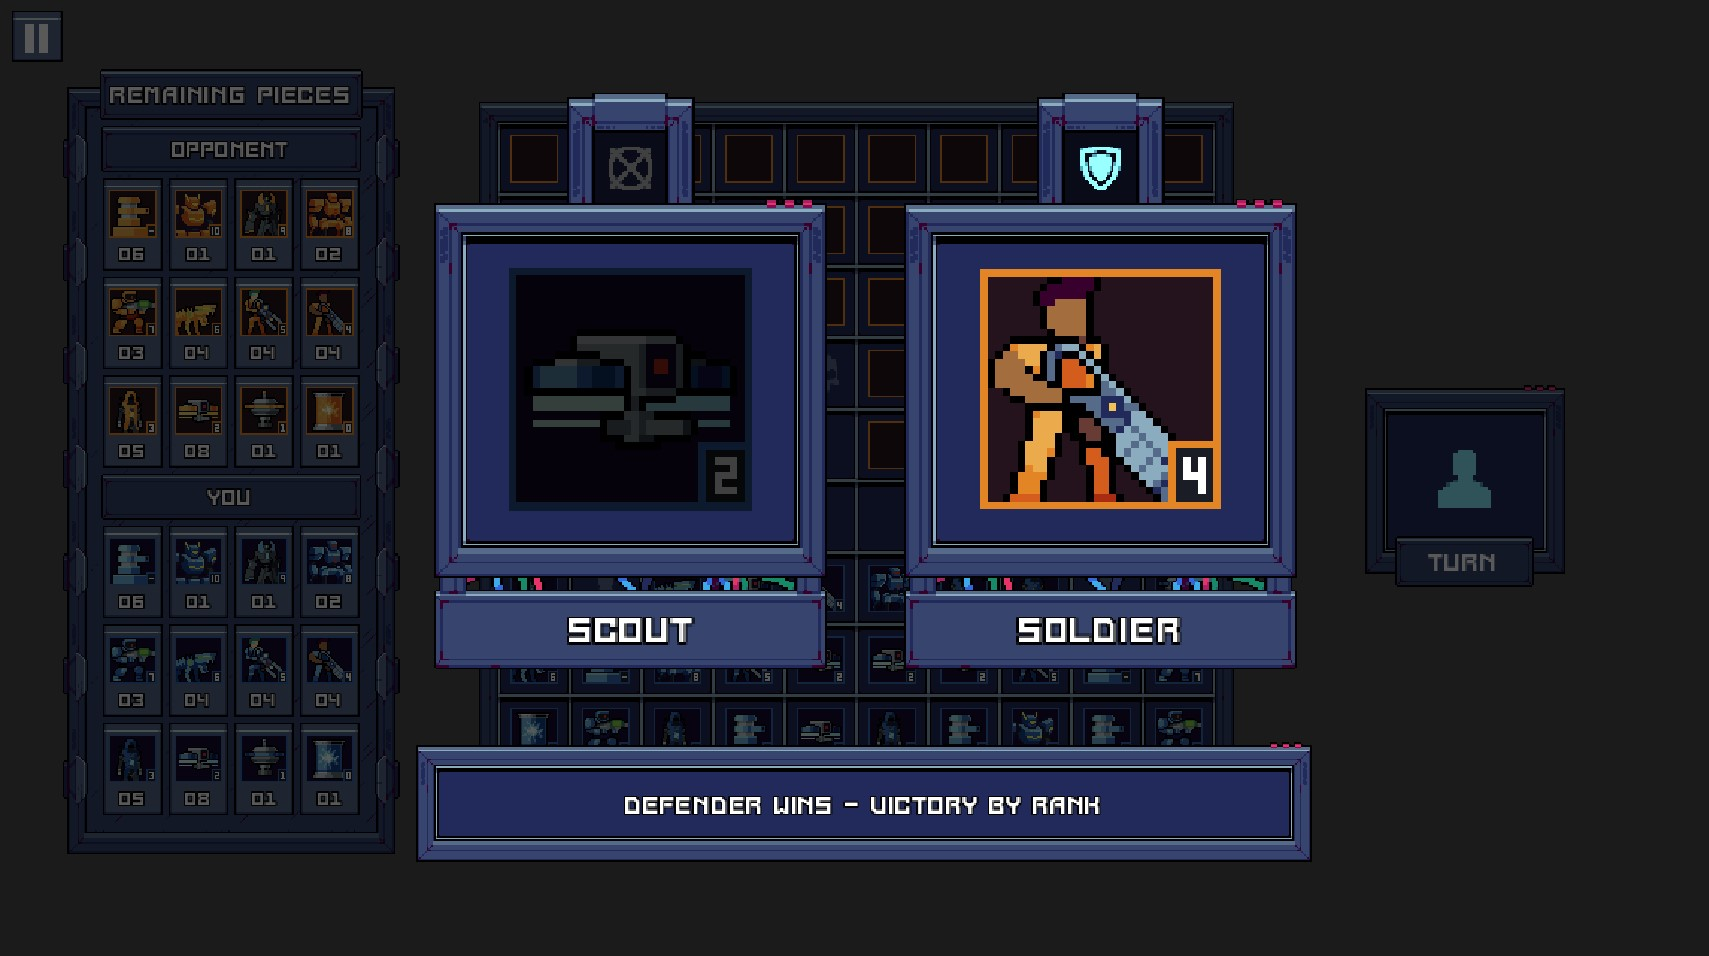
\includegraphics[width=\textwidth]{../Imagenes/MenuInterfazCombateResuelto}
	\caption{Interfaz de combate tras la resolución: pieza perdedora oscurecida
		y mensaje de resultado visible.}
	\label{fig:ManualMenuCombate}
\end{figure}

% ─────────────────────────────────────────────────────────────────────────────
\section{Menú de pausa}
% ─────────────────────────────────────────────────────────────────────────────

Durante el turno del jugador es posible pausar la partida pulsando la tecla \textit{Escape}. El menú de pausa ofrece cuatro opciones: \textit{Resume} para reanudar la partida desde el punto en que se pausó; \textit{Rules} para consultar las reglas sin abandonar la partida; \textit{Options} para acceder a la configuración de audio y visualización; y \textit{Return to Menu} para abandonar la partida en curso y volver al menú principal.

% ─────────────────────────────────────────────────────────────────────────────
\section{Menú de opciones}
% ─────────────────────────────────────────────────────────────────────────────

Accesible desde el menú principal y desde el menú de pausa, el menú de opciones permite cambiar el idioma del juego, alternar entre modo ventana y pantalla completa, y ajustar de forma independiente el volumen de los cuatro canales de audio disponibles: \textit{Master}, \textit{Music}, \textit{SFX} y \textit{UI}. Todos los cambios se aplican de forma inmediata. Para cerrar el menú se pulsa \textit{Go Back}.

% ─────────────────────────────────────────────────────────────────────────────
\section{Fin de partida}
% ─────────────────────────────────────────────────────────────────────────────

La partida termina cuando se destruye el núcleo de energía de uno de los bandos o cuando uno de ellos se queda sin piezas con capacidad de movimiento. La ventana de fin de partida (Figura~\ref{fig:ManualMenuFinPartida}) informa del resultado con un color que codifica el desenlace: verde para la victoria, rojo para la derrota y morado para el empate, indicando además el motivo concreto. Desde esta pantalla se puede iniciar una nueva partida pulsando \textit{Play Again} o regresar al menú principal pulsando \textit{Main Menu}.

\begin{figure}[H]
	\centering
	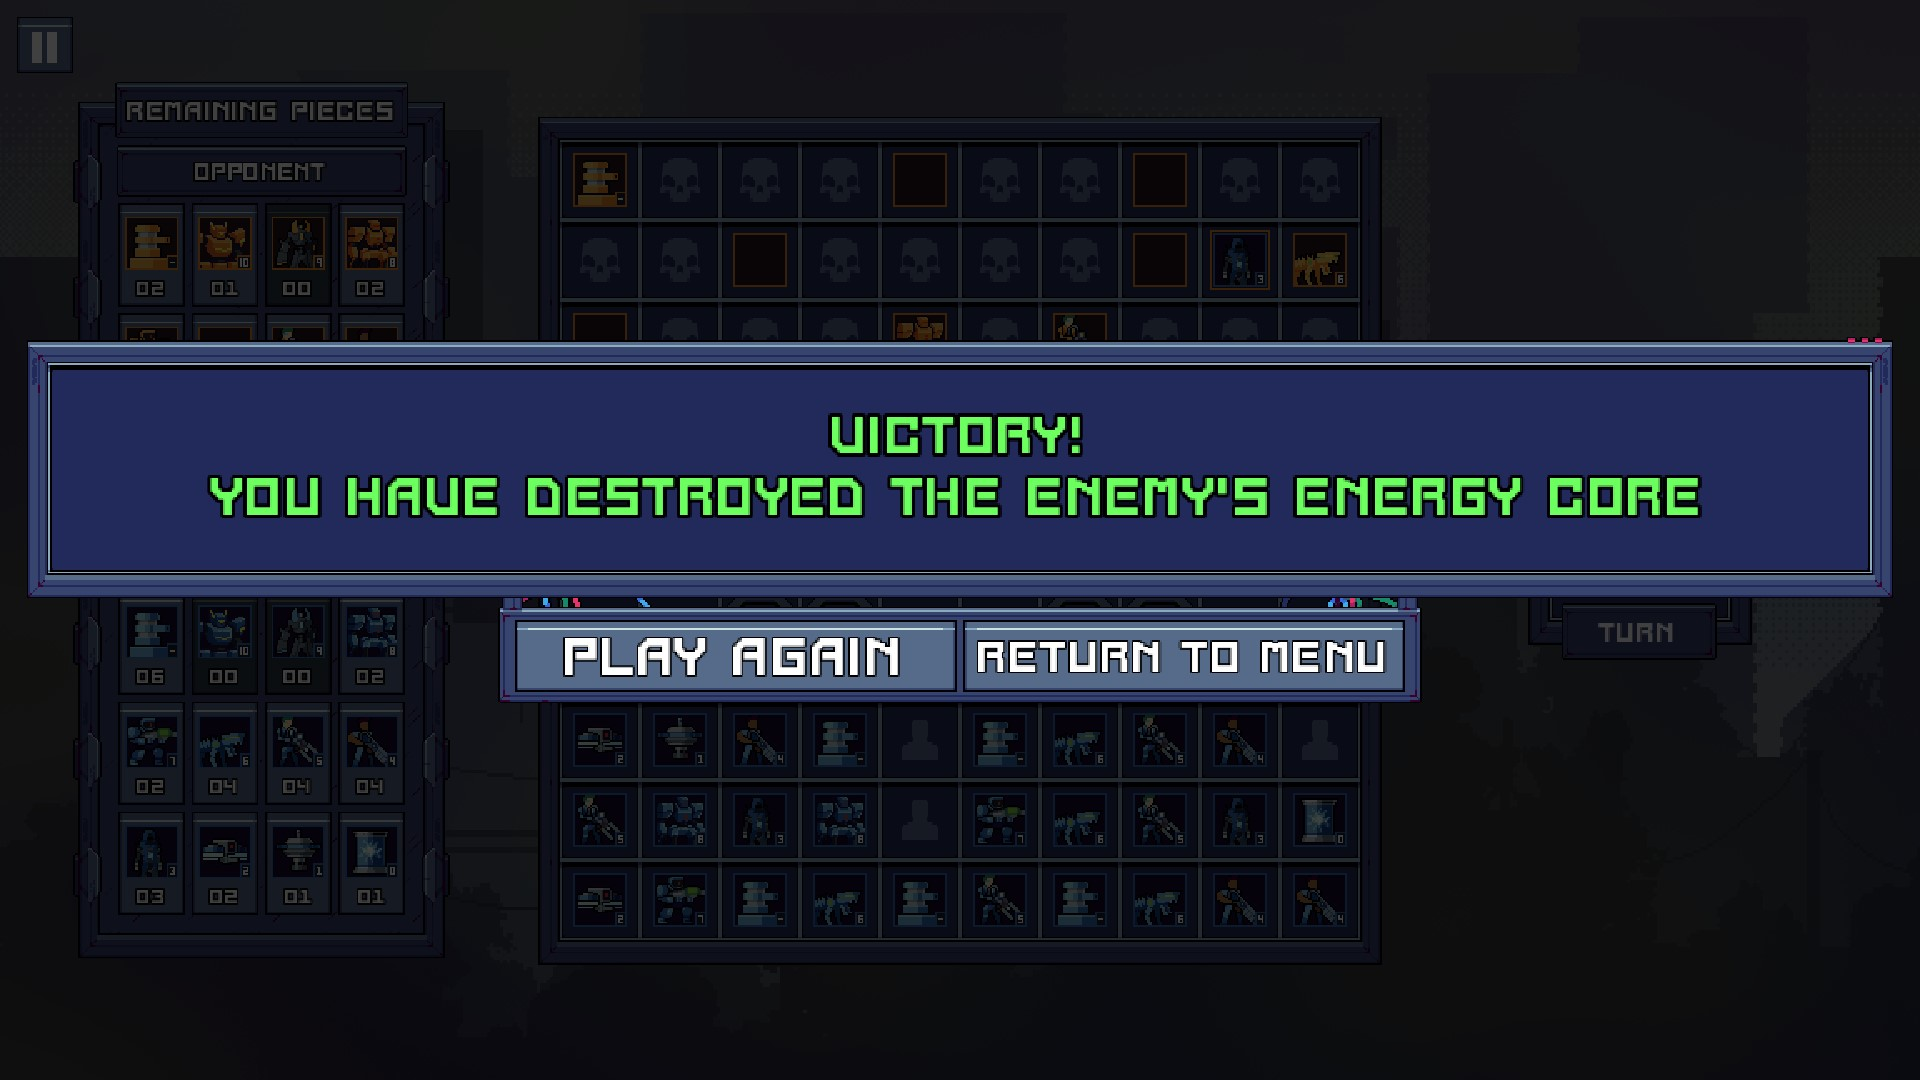
\includegraphics[width=\textwidth]{../Imagenes/MenuFinPartida}
	\caption{Pantalla de fin de partida con mensaje de victoria.}
	\label{fig:ManualMenuFinPartida}
\end{figure}